\documentclass[10pt, a4paper]{article}

\usepackage{a4wide}
\usepackage{listings}
\usepackage{comment}
\usepackage{amsmath}
\usepackage{graphicx}
\usepackage{url}
%\usepackage{hyperref}

\setlength{\parindent}{0pt}

\title{Symbolic Execution of Binary Code}
\author{SEASON Lab  \\
\url{season-lab.github.io} \\
Sapienza University of Rome  \\
}

\date{}

\begin{document}

\maketitle

\setcounter{tocdepth}{2}
\tableofcontents

\newpage
\section{Introduction}

Symbolic execution is a very powerful static analysis technique. In this paper, we describe the main aspects of this methodology and discuss how it has been extensively exploited in the context of computer security for analyzing binary code.

\section{Symbolic Execution}

Symbolic execution has been originally introduced in~\cite{K-ACM76} and~\cite{H-TSE77}. A good introduction to symbolic execution is present in~\cite{KLEE-OSDI08} (while~\cite{EXE-CCS06} is a previous effort of the same authors). \cite{SAGE-NDSS08} is one successful story of symbolic execution. \cite{SAB-SP10} is a clean formalization of symbolic execution (and taint analysis).

\subsection{Motivation}

Symbolic execution is a static analysis technique that have been introduced to perform automatic testing of complex software. For instance, consider the C function shown in Figure~\ref{fig:example-1}. A critical operation performed by this code is the division performed on line 10. Testing techniques such as random testing can generated several input tests for this function. However, it is unlikely that the inputs which make this code crash are effectively picked up by these techniques. Indeed, although this code is relatively simple, there are too many possible assignments to the input values {\tt a}, {\tt b}, and {\tt c}. In general, each {\tt int} input variable in C has $2^{32}$ possible values. In practice, only input values which lead to $x + y + z - 3$ equal to zero make the code crash.

Symbolic execution overcomes common limitations of random testing techniques by evaluating a piece of code using {\em symbols}, instead of concrete values for the inputs. The main idea is to consider classes of input values, instead of a single instance values. Before analyzing how symbolic execution can identify the proper inputs which will make the function {\tt foobar} crash, we need to introduce few basic definitions.

\subsection{A simple execution model}
\label{simple-execution-model}

Symbolic execution is a methodology for executing a program symbolically. At any point of the execution, a state is kept by the symbolic execution engine.

\paragraph{Symbol} Any local or global variable is associated to a symbol $\alpha_i$. 
\paragraph{Execution state} The execution state $(stmt,~pc)$ is composed by two kinds of information:
\begin{itemize}
  \item $stmt$: the next statement that should be evaluated
  \item $pc$: path constraints, i.e., set of assumptions made over the symbols $\alpha_i$ to reach the statement $stmt$. Initially the $pc$ is empty, i.e., set to true.
\end{itemize}
Since, in general, any memory location may have associated a symbol, it is common to maintain a memory mapping $M$ for storing constraints associated to different symbols.

\paragraph{Execution model} Depending on the kind of the statement $stmt$, the execution state is modified as follows:
\begin{itemize}
  \item (constant assignment) $\alpha_i = c$: when a constant value $c$ is assigned to a variable associated to the symbol $\alpha_i$, $pc$ is extended, adding the constraint:
    \[ pc \gets pc \wedge \alpha_i = c\]
  \item (assignment) $\alpha_i = e$: when an expression $e$ is assigned to a symbol $\alpha_i$, $pc$ is extended, adding the constraint:
    \[ pc \gets pc \wedge \alpha_i = e\]
  where $e$ can be any expression, such as unary or binary operation, over symbols and constants.
  \item (conditional branch) {\tt if} $e$ {\tt then} $stmt_{true}$ {\tt else} $stmt_{false}$: $pc$ is evaluated. Two scenarios are possible:
    \begin{itemize}
      \item (non-forking) $e$ is always verified (true) or always not verified (false): the proper branch is taken, evaluating $stmt_{true}$ or $stmt_{false}$.
      \item (forking) the boolean value of $e$ is not determinable without instantiating the values of one or more symbols: the symbolic execution is forked, creating two parallel execution states:
        \[ (stmt_{true}, pc_{true}) \text{ where } pc_{true} = pc \wedge e \]
        \[ (stmt_{false}, pc_{false}) \text{ where } pc_{flase} = pc \wedge \neg e \]
    \end{itemize}
    The execution is proceeded on both states.
  \item (jump) {\tt goto} $stmt$: the execution state is updated to match the given next statement to be evaluated. 
  \item (other constructs) A discussion of other constructs such as $call$, $return$, $while$, or $for$ is provided in Section~\ref{example-discussion}. 
\end{itemize}

\subsection{Example}
\label{symbolic-execution-example}

\begin{figure}[t]
\begin{lstlisting}[basicstyle=\ttfamily\small]
              1.  int foobar(int a, int b, int c) {
              2.    int x = 0, y = 0, z = 0;
              3.    if (a != 0)
              4.      x = -2;
              5.    if (b < 5) {
              6.      z = 2;
              7.      if (a == 0 && c != 0)
              8.        y = 1;
              9.    }
             10.    return a / (x + y + z - 3);
             11.  }
\end{lstlisting}
\label{fig:example-1}
\caption{Example: a very simple C function}
\end{figure}

\begin{figure}[t]
  \centering
  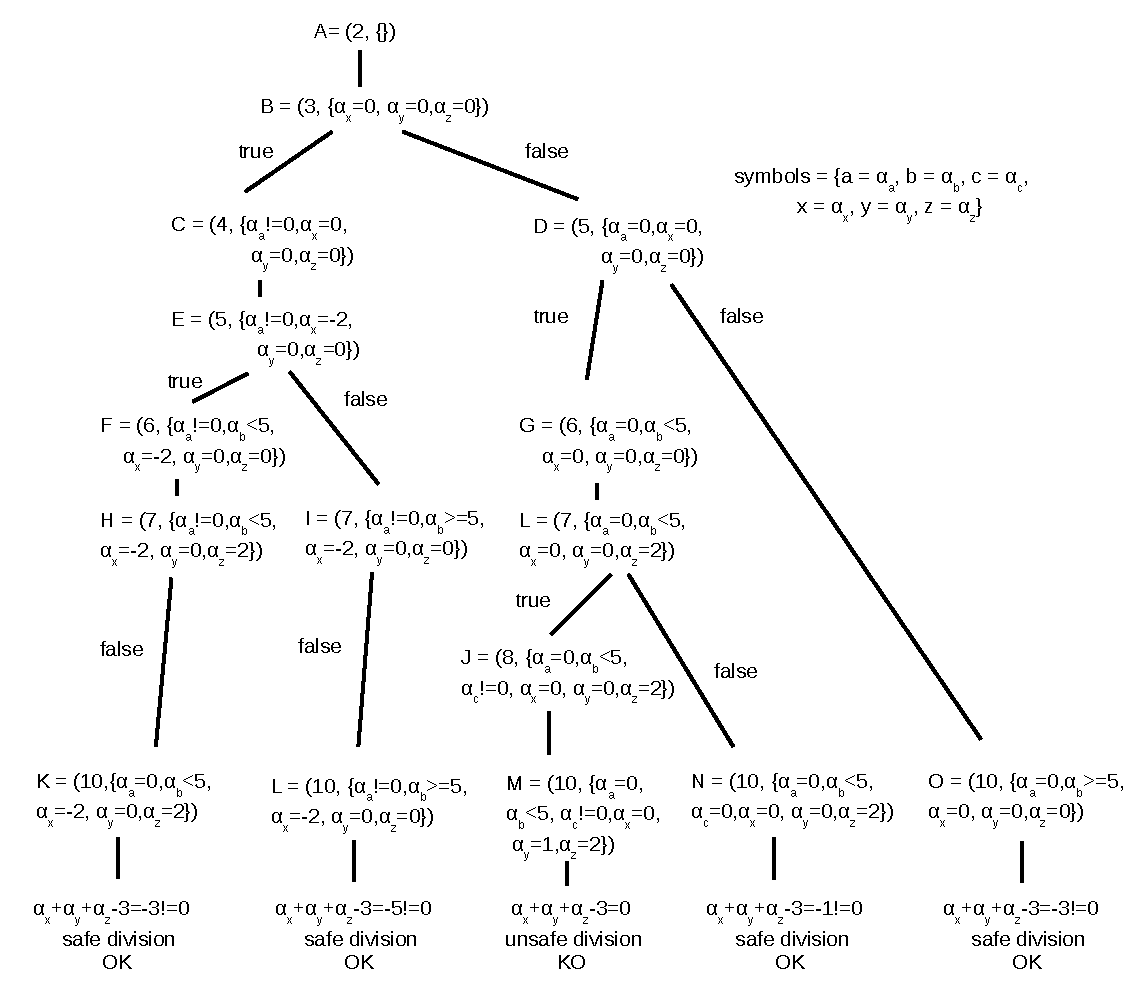
\includegraphics[width=1.0\columnwidth]{images/example} 
  \caption{Symbolic execution tree of the function {\tt foobar}. Each execution state is labeled with an alphabet letter.}
  \label{fig:example-symbolic-execution}
\end{figure}

The symbolic execution of the function {\tt foobar} is shown in Figure~\ref{fig:example-symbolic-execution}. Initially, a new symbol is introduced for each input argument and for each local variable. For the sake of the presentation, we have associated symbol $\alpha_{var}$ to the variable $var$. Moreover, we have assumed to know the set of local variables used by the function. In general, obtaining this information may be non trivial and thus it it common to introduce symbols related to local variables only when the statements defining the variables are evaluated. To track the mapping between variables and symbols, a mapping table is maintained. 

The first statement of the function is line 2. For this reason, the initial execution state $A$ is given by $(2, \{\})$ where the path constraint set is empty since no assumption can be made on any symbol. After executing line 2, the $pc$ is updated adding constraints on the value of $\alpha_x$, $\alpha_y$, and $\alpha_z$ (see execution state $B$). Line 3 contains a conditional branch: since the condition cannot be uniquely resolved based on the current set of assumptions, the execution is forked. Depending on the taken branch, a different statement is next evaluated and different assumptions are made on the symbol (see execution state $C$ and $D$). On the other hand, if the condition can be uniquely determined such as when evaluating the execution state $H$, then there is not need to fork the execution but it is sufficient to follow only the interesting branch (i.e., $K$), pruning away unrealistic execution states. 

After expanding any execution state until it reaches the statement on line 10, we can finally check which values for the input parameters {\tt a}, {\tt b}, and {\tt c} make the function {\tt foobar} crash by performing a division by zero operation. Analyzing execution states $\{K, L, M, N, O\}$, we can conclude that only the execution state $M$ lead to an unsafe operation. The path constraint set of $M$ defines the set of inputs which are unsafe for function {\tt foobar}: any input parameters for $\alpha_a$, $\alpha_b$, and $\alpha_c$ such that:
 \[ \alpha_x + \alpha_y + \alpha_z - 3 = 0 \wedge \alpha_a = 0 \wedge \alpha_b < \alpha_c \wedge \alpha_c \neq 0 \]

will crash this function. An instance of unsafe input parameters for {\tt foobar} can determined exploiting a constraint solver (i.e., an oracle able to resolve constraints). For instance, a solver may come up with the values $a = 0$, $b = 1$, and $c = 2$ given the execution state $M$. Notice that a constraint solver is also needed when evaluating the satisfiability of branch conditions. 

\subsection{Discussion}
\label{example-discussion}

The example described in Section~\ref{symbolic-execution-example} shows the effectiveness of the symbolic execution methodology in finding {\em all} the possible unsafe input values which may trigger a crash given by the division performed on line 10. This is achieved by symbolic execution through an exhaustive exploration of all the possible execution states. For this reason, at least from a theoretical point of view, symbolic execution can be seen as a sound and complete approach. This means that if an input values is detected as unsafe then it is actually unsafe. Moreover, symbolic execution is able to always find all the unsafe inputs. However, several observations and questions naturally arise:

\begin{enumerate}

  \item (objects) {\em How does symbolic execution handle arrays or other more complex objects?} \\
  In general, any arbitrary complex object can be seen as an array of bytes, where each byte can have associated a distinct symbol. Indeed, even a C {\tt int} type can be seen as an array of four bytes. In practice, it is convenient, whenever possible (e.g., by statically analyzing the source code), to exploit structural properties of the data. 

  \item (loops) {\em How does symbolic execution handle loops?} \\
  Using the execution model presented in Section~\ref{simple-execution-model}, a loop can be evaluated by translated it into a combination of conditional branches and $goto$ statements. This transformation is not uncommon when a high-level language like C is compiled into binary code. However, the main critical aspect when symbolically executing a loop is choosing how many iterations should be analyzed. In general, a loop may be repeated depending on the value of some variables whose values may be not constant, e.g., the number of iterations is given by the value of an input parameter. The naive approach can lead to create a new execution state for each possible repetition of the loop.

  \item (subroutines) {\em How does symbolic execution handle subroutines?} \\
  The execution model presented in Section~\ref{simple-execution-model} does not specify how to handle invocation to subroutines (i.e., a $call$ statement). An way to extend our execution model in order to handle subroutines it to expand the execution state by adding a simple execution stack.

  \item (recursion) {\em How does symbolic execution handle recursion?} \\
  Consider, as an example, the code:
    \begin{lstlisting}[basicstyle=\ttfamily\small]
    1.  int bar(int n) {
    2.    if (n >= 0) 
    3.      return 0;
    4.    return 1 + sum(n - 1);
    5.  }
    \end{lstlisting}
  Assuming to have introduced an execution stack in the execution state, it can be easily observed that the above can easily lead to a very large number of executions states. Indeed, the number of executions states is related to the number of times that the conditional branch on line 2 is not taken. 

  Since the {\tt int} type in C can have $2^{31} - 1$ positive values, symbolic execution has to create more than $2^{31} - 1$  execution states to cover all the possible execution paths.
 
  \item (environment) {\em How does symbolic execution handle interaction with the environment}? 
  Real-world applications interacts constantly with the environment: this is typically achieved by invoking library or system routines. A crucial aspect of these interactions is that they may cause some side-effects on the environments (e.g., creation of a file or initialization of a memory area) which must be considered since they may affect the actual execution of the code. Evaluating any possible outcome of an interaction is not feasible in most scenarios due to the large number of execution states which could be required. Moreover, it is likely that only a very small subset of this outcome is actually realistic. Hence, it is common to create models for popular library and system routines that help the symbolic execution engine to consider only significant outcomes.

  \item (state space explosion, path selection) {\em How does symbolic execution deal with path explosion}? \\
  A relatively simple code such as function {\tt foobar}, which is composed by less 12 lines of code, has generated 16 execution states, where $5$ out of $16$ are independent and must be checked to determine possible unsafe input values. Although this could seem a reasonable number of states, few lines of code, such as loops, may contribute to exponentially increase the number of states. For this reason, it is unlikely that a symbolic execution engine is able to exhaustively explore all the possible execution states within a reasonable amount of time. In practice, several heuristics must be exploited to prioritize evaluation of some states, hoping to still be able to spot interesting things. Moreover, the symbolic execution engine should include efficient mechanism for efficiently evaluating in parallel different execution states without running out of computational resources.

  \item (constraint solver) {\em What is a constraint solver in practice}? \\
  Constraint solvers exist in practice but they have significant limitations. A common limitation is that they are able to solve complex constraints in a reasonable amount of time only if these constraints are composed by linear expression over the symbols $\alpha_i$. For this reason, it is common to integrate optimizations in the symbolic execution engine that are able to generate {\em solver-friendly} constraints.

  \item (binary code) {\em What are the disadvantages of symbolically executing binary code}? \\
  The example presented in Section~\ref{symbolic-execution-example} is written in C. This does not mean that symbolic execution cannot be performed directly on binary code. However, having the source code of an application can significantly make it easier its symbolic execution since several sound assumptions can be obtained by statically analyzing the source code (e.g., the maximum size of a buffer or the number of iterations for a loop).
   
\end{enumerate}
Depending on the specific application context of symbolic execution, different choices and assumptions are made to address the above questions. Although soundness and completeness of symbolic execution may be negatively affected by these choices, there are several application scenarios where a partial exploration of the possible execution states is enough for reaching the ultimate goal (e.g., identify a single input that crashes an application).

\subsection{Memory model}
\subsection{Loops}
\subsection{Interaction with environment}

\subsection{State space explosion}


\subsubsection{Kinds of executors}
A symbolic execution engine should guarantee three main principles (\cite{MAYHEM-SP12}):
\begin{enumerate}
  \item the system should be able to forward progress for arbitrarily long times, ideally forever, without exceeding the given resources
  \item to maximize performance, no work should be repeated
  \item the system should reuse as much as possible previous analysis results
\end{enumerate}

Based on these principles, symbolic executors can be divided into:
\begin{itemize}
  \item {\em offline} executors (e.g., \cite{SAGE-NDSS08}): one path at time, every run independent from the others, results can be immediately reused, each run restart the execution of the program from the beginning. In order to perform a run, two inputs must be provided: the target program and a seed input. The program is concretely executed and a trace is recorded. Then the trace is symbolically executed. This is can be seen as a way of {\em concolic} execution.
  \item {\em online} executors (e.g., \cite{KLEE-OSDI08,CKC-TOCS12,AEG-NDSS11}: for each fork, the execution state is cloned. All active execution states are kept in memory, no need to re-execute but huge burden on memory resources. A form of {\em context switch} is often needed. Execute may stop forking at a certain point to allow progress, but then some path are ignored. Memory is saved by aggressive copy-on-write optimization (e.g., immutable state). DFS can be used as exploration strategy in order to minimize memory consumption but can be very slow at doing progress. Notice that since multiple runs may be executed in parallel, isolation must be guaranteed (e.g., keeping different states of the OS by emulating system calls).
  \item {\em hybrid} executors (e.g., \cite{MAYHEM-SP12}): mixed approach. Start with an online approach, if needed switch to offline mode by doing checkpoints. A checkpoint contains the symbolic execution state and replay information. Concrete execution state is discarded since it can quickly recovered at runtime by using one input generated by solver before checkpointing.
\end{itemize}

\subsection{Path selection (aka state scheduling)}
Different heuristics can be used for deciding which execution state should be evaluated:
\begin{itemize}

  \item \cite{AEG-NDSS11}:
  \begin{itemize}
    \item {\em buggy-path-first}: priority to path that shown to contain errors (even if not exploitable)
    \item {\em loop exhaustion}: give priority to path that are exhausting a loop. In practice this can hit exploitable bugs (buffer overflows), but can prevent progress. Allow only one executor that is exhausting a loop, aggressive preconditioned symbolic execution.
  \end{itemize}

  \item \cite{KLEE-OSDI08} interleaves in a round robin fashion these strategies:
  \begin{itemize}
    \item {\em random path selection}: build a binary tree structure of all the state (each state is always create due to a fork from a parent). Assign same probability to be executed among states of the same subtree. Avoid starvation by given priority to states high in the tree.
    \item {\em coverage optimize search}: assign weights based on how much new code has been covered by a path. Pick up state randomly using weights as probability.
  \end{itemize}
  Each state is executed only for time slice defined both as maximum number of instructions and as maximum amount of time.

  \item \cite{MAYHEM-SP12} same heuristics as~\cite{SAGE-NDSS08} and~\cite{KLEE-OSDI08}:
  \begin{itemize}
    \item executors exploring new code have high priority
    \item executors that identify symbolic memory accesses have high priority
    \item executors where symbolic instruction pointers are detected have high priority
  \end{itemize}
\end{itemize}

\subsection{Constraint solvers}
\subsection{Challenges given by symbolic execution of binary code}

\section{Literature on symbolic execution}

\subsection{\cite{K-ACM76} Symbolic execution and program testing} 

\subsubsection{Goal}

Test a program using symbols, not actual inputs, which represents a class of inputs (determined by the dependence of the program's control flow on its inputs).

\subsubsection{Approach}     
  \begin{itemize}   
    
    \item inputs are seen as symbols ${\alpha}_i$ (integers)
    
    \item execution state:
      \begin{enumerate}
        \item current statement executed
        \item path condition (pc): 
          \begin{itemize}
            \item set of assumptions over inputs made to reach the current statement
            \item initially set to true
          \end{itemize}
      \end{enumerate}

      \item {\tt IF}: when there is a branch: 
        \begin{lstlisting}
      if q
          then ...
          else ...
        \end{lstlisting}
        where q can be any kind of expression over ${\alpha}_i$. Check q, if always false or always true, proceed with
        execution (non forking) and do not alter pc. Otherwise, perform forking by expanding in parallel two branches:
        \begin{enumerate}
          \item pc $\gets$ pc $\wedge$ q (condition satisfied)
          \item pc $\gets$ pc $\wedge$ !q
        \end{enumerate}
        proceed with execution on both branches. pc always remains true.

  \end{itemize}

\subsection{\cite{H-TSE77} Symbolic Testing and the DISSECT Symbolic Evaluation System} 

  \subsubsection{Goal} 
  Improved symbolic execution engine wrt~\cite{K-ACM76}.

  \subsubsection{Approach}

    \begin{itemize}
      \item input commands: if there is a loop with an input instruction (e.g., read) then label the symbol with the path index (index in the execution tree):

        \begin{lstlisting}
      1. for i=1 to N 
      2. x = read(...)
        \end{lstlisting}
      Then:
      \begin{lstlisting}
      x = x:2 (when i=1)
      x = x:4 (i=2)
        \end{lstlisting}

        \item output commands and variable values: problems due to array reference, e.g.:
      \begin{lstlisting}[mathescape=true]
    1. X = array(10)
    2. I = 2
    3. X(I) = 0 $\Rightarrow$ X(I:2) = 0
    4. I = read()
    5. X(I) = 10 $\Rightarrow$ X(I:4) = 10
    6. Y = X(2)
      \end{lstlisting}
      Y is X(2):5 meaning that is the value assigned at the path index 5 or an earlier value assigned to it. To keep track of earlier values, we keep a list of values related to values(X(2)) = \{0, X(2):5\}

      \item users can use some path selection commands to indicate which branches are taken, how many time a loop is executed, add branches, halt

    \end{itemize}

\subsection{\cite{KLEE-OSDI08} KLEE: Unassisted and automatic generation of high-coverage tests for complex systems programs} 

\subsubsection{Goal}

Symbolic execution engine for generating code coverage tests for C applications.

\subsubsection{Approach}

KLEE does not currently support: symbolic floating point, longjmp, threads, and assembly code. Additionally, memory objects are required to have concrete sizes.

KLEE works on the LLVM bytecode generate by LLVM-gcc. Given as input the bytecode, it generates inputs (constraints can be put on the number of cmd arguments, their maximum length, maximum times syscall can fail), Tests can be run on actual code, generated with native compiler. Input marked as symbolic have associated a constraint on it (initially this could be nothing). When a conditional is met in the code, a constraint solver determines which branch is taken. If current constraints do not lead to a specific branch, then there is an execution fork. When a bug (exception, memory error) or process exit is hit, the constrain solver is used to obtain valid inputs which lead to that exit point. KLEE analyzes the bytecode and modifies the state based on the side effects given by a statement. If a fork is needed, the state is cloned and a new KLEE process is instantiated. If a load/store works on an address which could point to different objects, for each object a fork is executed and the address is bounded to that object from now on. Memory is not seen as a single array, but divided in many objects (stack, heap objects, etc.) and copy on write is used to minimize overhead due to cloning (e.g., cloning heap has constant cost).

Some aspects:

\begin{itemize}

  \item Process scheduling: Need to decide what is the next KLEE process to run. Different strategies:
    \begin{itemize}
      \item random: a tree is build where internal nodes are branch points, and leaves are the active KLEE processes. A random path is chosen. Notice that all leaves under the same branch point get the same probability to be executed. Properties:
        \begin{enumerate}
          \item avoid starvation (too many forks in one region)
          \item favor nodes high in the tree, which are relatively unconstrained
        \end{enumerate}
      \item uncovered regions: choose process using some heuristics. which can cover uncovered code. Assign weight to each process based on the min distance to uncovered code, consider stack, consider whether that region has recently covered uncovered code. Then pick randomly.
    \end{itemize}
    Each process is executed for time-slice, which is based on the cost of the statement Indeed, expensive instructions should not dominate the execution otherwise limited progress is done.

  \item Query optimization: KLEE spends most of the time querying the constraint solver. Hence, query optimization is crucial. Techniques:
    \begin{itemize}
      \item constraint independence: divide constraints in independent disjoint subsets based on the symbolic variables which they reference. Irrelevant constraints can detected and discarded.
      \item counterexample caching: keep a cache of counterexample based on past queries:
        \begin{itemize}
          \item if a subset of constraints has not solution, any superset does not have as well
          \item if a superset has a solution, any subset has a solution
          \item if a subset has a solution, try it for the superset
        \end{itemize}
    \end{itemize}
  \item Interaction with environment. Invocation to syscalls are replaced with invocations to models. Each model wraps a syscall (e.g., read) and can either just invokes the real syscall or emulated it with a symbolic variant. Whether bind to real or symbolic syscall, it is decided during open() or similar syscall: e.g., if the filename is constant then the actual file is opened, otherwise (i.e., the filename is symbolic) a symbolic file is returned. Notice that:
            \[ \text{open(argv[1])} \]
  will bind to symbolic file and add constraint on argv[1] that specifies that argv[1] is a filename. Notice that a symbolic open() will fail one time and N parallel KLEE processes will be added: one for each possible symbolic file specified by the user (e.g., different sizes, different permissions, they are actual files passed by the user in a specific directory). Hence, N+1 branches are created for a symbolic open(). For efficiency, a symbolic open() will generate only 2 branch: one for covering the fail, and one matching all available symbolic files. Only when needed, this branch is exploded. Notice that syscall failure is covered both for realistic cases (e.g., file not exists) and for uncommon scenarios (e.g., write failure due to no available disk space). Uncommon scenarios can be disabled for efficiency. Notice that when tests are generated, if needed, symbolic files are instantiated using the files specified by the user for the symbolic syscall. Failure of syscall are reproduced during real tests (executed without KLEE) exploiting ptrace.

\end{itemize}

\subsection{\cite{EXE-CCS06} EXE: Automatically Generating Inputs of Death} 

\subsubsection{Goal}
Identify inputs that may crash an application

\subsubsection{Approach}
Custom made constraint solver called STP, available at https://github.com/stp/stp\\


Does not handle floating point values. User must mark all the variable which should be considered as symbolic. CIL is used as source-to-source translator, its output is then compiled with gcc. EXE exploits CIL to propagation of constraints, fork execution if needed,  call STP when execution is finished (e.g., exception, exit, error) and symbols must be instantiated in order to get a valid test. Assertion violations are seen as errors.

Some aspects:
\begin{itemize}
  
  \item STP is a decision procedure for bitvectors and arrays. Instead of using the Nelson-Open's cooperating decision procedures framework, they built STP based on th experience of a previous work called CVCL. Using mathematical and logical identities, constraints are translated in purely propositional logic formulae that are fed to the MiniSAT solver. The code of STP is smaller than CVCL. Data are always seen as untyped. Any operation is mapped to bitvectors. x + y is a bitvector operation, while x + y < z is a formula. Formula are translated in DAGs of single bit operations. 

  \item Each symbolic data is represented as as an array of 8-bit vectors. For each object b of size $|b|$ which is marked as symbolic by the user, EXE create an array $b_{sym}$ of size $|b|$ and track this mapping in a table. Other mappings are added to the table due to an assignment (v = e) or reference to an element of an array (b[e]) (b is imported in STP as an array of the same size).

  \item Construction of an expression e: if there is a read of area of size n, then EXE check if that area is concrete. In this case, the concrete values are inserted in e. Otherwise, e is bind to the concatenation of $b_1,..., b_n-1$. For each distinct byte, if it is concrete, then its value is used. Otherwise, it uses it symbolic expression $(b)_i$. E.g.  $a + i*4$ where a is the starting addr of an array and i an integer of four bytes, then the result is:
    \[ a + (i_sym[3] + i_sym[2] + i_sym[1] + i_sym[0]) * 00...0100 \]

  \item Pointer are seen as array reference at some offset. For this reason, allocation and deallocation are tracked. Double references like **p force to STP concretize *p, fixing a storage location.

  \item Fast array constraints: few translations are needed in order to make STP faster. FTP works on purely functional language:
    \begin{lstlisting}
      // read value v at position i in A
      v  = read(A, i)      
      
      // write on a copy of A, v at A[i]
      A' = write(A, i. v)  
      
      // if condition then a else b
      ite(condition, a, b) 
    \end{lstlisting}
      STP removes any write (note: any write makes sense only if there is a subsequent read):
    \begin{lstlisting}[mathescape=true]
      read(write(A, i, v), j) $\implies$ ite(i == j, v, read(A, j))
    \end{lstlisting}
      STP removes and read, by enforcing that if you read from the same location twice, then you get the same value:
    \begin{lstlisting}
      (read(A, i) = e_1)  and (read(A, j) = e_2)
    \end{lstlisting}
    will be transformed in:
    \begin{lstlisting}[mathescape=true]
      (v_1 = e_1) and (v_2 = e_2) and (i $=$ j $\implies$ v_1 = v_2)
    \end{lstlisting}
  Notice that these techniques increase the size of the formula. For this reason, other optimizations are needed. Array substitution optimization substituting out all constraints of any read(A, c) = e where c is constant:
  \begin{enumerate}
    \item read(A, c) $\implies$ e
    \item ???
  \end{enumerate}
  STP perform lazy evaluation of array refinement: e.g., do not consider some axioms, find solution, see if satisfiable in the original formula then ok, otherwise add some axioms (not all) and then re-evaluate, repeat if needed.

\end{itemize}

\subsection{\cite{SAGE-NDSS08} Automated white-box fuzz testing} 

\subsubsection{Goal}
Use symbolic execution for performing white-box fuzz testing. This paper is especially important because SAGE (the tool presented in this paper) has been extensively used at Microsoft.

\subsubsection{Approach}
Fuzz testing is typically a black-box approach: random inputs are generated and execution is monitored to check errors and unexpected behaviors. Unfortunately, it is unlikely to cover the whole code with random inputs. They propose to exploit symbolic execution to perform fuzz testing.

It works on x86 binaries, exploits Dissolver (a distributed solver), iDNA (to trace execution), and TruScan (to virtually play traces). 

Main aspects:
\begin{itemize}
  \item Generational search: initially starts with a seed input and bound set to zero
    \begin{lstlisting}[mathescape=true]
  check input I for errors (concrete execution, if error than: 
    generate a trace + replay trace for listing executed BB)
  generate symbolic constraints (using the trace)
  childInputs = []
  for (i = bound, i < |constraints|, i++)
    set constraints[bound, ..., i - 1] to true 
      (i.e., exploit concrete input values)
    set constraints[i] to false (possibly this will affect input)
    solve constraints, if SAT:
      create new input I' by updating I
      set bound of I' to I
      add I' to childInputs 
  for each child input, execute (1), compute a score
   based on the number of previously uncovered BBs
  sort child inputs based on score
  for each child input, restart from beginning 
    \end{lstlisting}
    \item SAGE maintains concrete and symbolic states using (value, tag). Tag can be:
      \begin{itemize}
        \item input(m): m-th byte of the input
        \item c: constant
        \item t1 op t2: binary op over two tags: e.g., a concatenation of two tags (e.g., useful to handle registers like cx = (t\_ch, t\_cl))
        \item subtag(t, i): i-th byte of the tag t
      \end{itemize}
    \item Constraint optimizations:
      \begin{itemize}
        \item tag caching
        \item unrelated constraint elimination
        \item local constraint caching
        \item flip count limit
        \item constraint subsumption
      \end{itemize}
\end{itemize}

\subsection{\cite{SAB-SP10} All You Ever Wanted to Know About Dynamic Taint Analysis and Forward Symbolic Execution (but might have been afraid to ask)}

This a formalization of symbolic execution and taint analysis.

\section{Literature on concolic execution}

Concolic execution has been introduced by~\cite{DART-PLDI05} and later improved by~\cite{CUTE-FSE13}. Notice that concolic execution can be seen a symbolic execution where constraints on the inputs lead to single input instance.

\subsection{\cite{DART-PLDI05} DART: directed automated random testing}

\subsubsection{Goal}

Automatically generate random tests

\subsubsection{Approach}

{\bf Problem:} symbolic execution can hit non linear constraints.\\
{\bf Idea:} do symbolic execution, if needed, perform also concrete evaluation.\\


Three main steps:
\begin{enumerate}
  \item automated extraction of program interfaces. Three kinds of functions:
    \begin{itemize}
      \item program (code)
      \item external functions: routines controlled by the environment and that can be non deterministic. Dart will wrap them and return random results. Assumed that they do not perform any side-effect. Otherwise, they should be simulated.
      \item library functions: not in code, but still deterministic
    \end{itemize}
  \item automatic generation of random tests:. Inputs are generated randomly
  \item dynamic analysis of the program behavior under random testing with automatic generation of new test inputs to direct systematically the execution along alternative program paths
\end{enumerate}

Execution model:
\begin{itemize}
  \item P: the program executed both concretely on random input and symbolically. P execute statements (stored at specific locations $l_i$). which can manipulate the memory.
  \item M: memory (context), a mapping from memory addresses to, for instance, 32-bit words
  \item M' := M + [m -> v]: update of M where M'[m] = v. where m can be an address or a symbolic variable
  \item e: symbolic expression (no side effect!)
    \begin{enumerate}
      \item m: address or symbolic variable)
      \item constant
      \item *(e', e''): multiplication
      \item <=(e', e''): comparison
      \item !(e'): negation
      \item *(e'): deference
    \end{enumerate}
  \item statement at $l_i$:
    \begin{enumerate}
      \item label l: address of another statement
      \item conditional c: if (e) then goto $l_k$
      \item assignment a: m $\gets$ e where m is an address
      \item abort or halt
    \end{enumerate}
  \item evaluate\_concrete(e, M): evaluate e in context M and return a 32-bit value for e
  \item statement\_at(l, M): next statement to be executed at l. If assignment, returns the address where to save the right hand side
  \item input addresses $M_0$: addresses of input parameters for P
  \item input vector I: initial values for values in $M_0$, which gives M (initial context)
  \item A: set of conditional statements
  \item C: set of conditional statements
  \item EXECS := (A u C)* (halt $|$ abort)
  \item program execution w: a finite sequence in EXECS. which can written as:
  
    \[ alpha_1~c_1~alpha_2~c_2~[...]~alpha_{k+1}~s \]
    where:
      \begin{itemize}
        \item $\alpha_i$ in A*
        \item $c_i$ in C
        \item $s \in$ {halt. abort}
      \end{itemize}
      Notice that given I, then w can be determined.
    \item EXECS(P): subset of EXECS valid for P given all possible I. This can be represented as an execution tree, where assignments have one successor, conditionals have one or two successors, leaves are (halt $|$ abort)

\end{itemize}

\subsection{\cite{CUTE-FSE13} CUTE: a concolic unit testing engine for C} 

\subsubsection{Goal}
Efficiently test code

\subsubsection{Approach}

\begin{enumerate}
  \item create a logical input map I that represents all inputs
  \item using I, generates a concrete graph memory for the program
  \item create two symbolic states: one for pointer values and one for primitive values
  \item runs the code on the concrete graph memory, collecting constraints on symbol variables: CUTE finds all the inputs that follows the same path generated by the current concrete inputs
  \item negates constraints to obtain a new logical input map I' which likely can lead to a different path
  \item repeat from (1) using I'
\end{enumerate}


Notice that when a constrain cannot be solve, the concrete value is considered. If due to this, some path cannot be explored (the concrete value always lead to the same branch) then a new execution of CUTE is started where other random inputs are used as concrete values.

Notice that if a functions takes as input a data structure then two approached can used:
\begin{itemize}
  \item exploit a chain of calls for initializing the data structure
  \item exploit data structure invariants specified by the user through few notations
\end{itemize}

Simple constraints are set on pointer:
\begin{enumerate}
  \item equal or not equal to another pointer
  \item NULL or not NULL
\end{enumerate}

\section{Applications}

\subsection{\cite{FIRMALICE-NDSS15} Firmalice - Automatic Detection of Authentication Bypass Vulnerabilities in Binary Firmware} 

\subsubsection{Goal}
Analyze a firmware and detect auth bypass inside it.

\subsubsection{Approach}

Steps:
\begin{enumerate}
  \item Firmware loading: 
    \begin{itemize}
      \item disassembly: they assume that the blobs are not excessively obfuscated or ciphered. If they are then [KRV-USENIX-SEC15]
      \item base address determination: analyze jump table (referred by indirect jumps)
      \item entry point discovery: build call graph, consider root nodes of weakly connected components
    \end{itemize}
  \item Security policies: user should define when bypass occurs e.g., if code reach auth success string, actions (read by a device), reserved memory areas, privileged code
  \item Static program analysis:
    \begin{itemize}
      \item build context sensitive CFG exploiting a symbolic execution engine for resolving jumps
      \item build control dependency graph (CDG), obtained by transforming CFG
      \item build data dependency graph (DDG) that shows how instructions correlate wit each other with respect to the production and consumption of data. Obtained by using data flow analysis approach in [TG-CC06]
      \item backward slicing: given a program point produce every statement on which that point depends. Slicing technique from [KJL-SCAM03]. Creation of authentication slice (analyze all code is costly).
    \end{itemize}
  \item Symbolic exec engine to find inputs to reach privileged code. Concepts from~\cite{KLEE-OSDI08} [FUZZBALL-SSTA11] \cite{MAYHEM-SP12}.
    \begin{itemize}
      \item used Z3 as constraint solver
      \item symbolic summaries: instead of analyzing all subroutines, tries to model common routines (e.g., libc) and detect them in blobs. Several test cases that check pre/post conditions.
      \item lazy initialization: if there is a read over uninitialized data, then identify writes to that area, analyze path with and without initialization
    \end{itemize}
  \item  Authentication bypass check: analyze inputs that reach s code, if not concrete generate a function that can generate them. Also identify data exposed.
\end{enumerate}

\subsection{\cite{MAYHEM-SP12} Unleashing MAYHEM on Binary Code} 

\subsubsection{Goal}
Automatically generate exploit for a binary.

\subsubsection{Approach}      
MAYHEM has two core parallel components:
\begin{enumerate}
  \item CEC: concrete execution client
  \item SES: symbolic execution server
\end{enumerate}

Steps:
\begin{enumerate}
  \item users specify class of input parameters
  \item CEC loads the binary, instruments the code, and performs dynamic taint analysis, detecting for each block of instruction, which are tainted and have impact on the flow (cjmp or call). When this is detected by CEC, the execution is suspended and block is sent to the SES
  \item Instructions are translated by the SES into an intermediate language using [BAP-CAV11] and keep track of concrete values (provided by CEC). SES maintains two kinds of formula:
  \begin{itemize}
    \item path formula: condition on symbols that lead to the current path
    \item exploitable formula: it determines if the attacker is able to:
    \begin{itemize}
      \item modify EIP
      \item execute a payload
    \end{itemize}
  \end{itemize}
  If needed the SES forks execution and the informs CEC the branch where continue the concrete execution. If the resources cap is reached, then, instead of actually forking, a checkpoint is created. A checkpoint is a way to save partial state (only symbolic state is saved, not concrete) to disk and restore it when resources are available. To restore concrete execution, the symbolic state is exploited (e.g., choose input values).Copy on write is used to take snapshots efficiently.
  \item if there is a tainted jump then MAYHEM builds an exploitable formula and uses the solver to check whether it is satisfiable. If exploit found, then the goal is reached. Otherwise, explore other paths.
\end{enumerate}

Other aspects:
\begin{itemize}
  \item A virtualization layer is needed to isolate different concrete executions and hide their side effects
  \item MAYHEM uses precondition symbolic executions, hints by user which restricts the solution space for symbols and thus help the symbolic execution engine.
  \item MEYHEM uses an index-based memory model:
    \begin{itemize}
      \item $\pi : I \to E$ where i is a 32-bit index in I, e is an expression in E 
      \item $e \gets load(\pi, i)$ where i indexes memory $\pi$, e represents the contents of the i-th memory cell
      \item $store(\pi, i, e)$: a new memory is returned
    \end{itemize}
    Unfortunately, fully symbolic memory is not scalable. Concretizing any memory operations is too limiting in practice. For this reason, MAYHEM models memory partially:
    \begin{itemize}
      \item writes are always concretize
      \item reads are allowed to be modeled symbolically
    \end{itemize}
    To make this efficient, several techniques are adopted: 
    \begin{itemize}
      \item upper and lower bounds on reference
      \item value set analysis
      \item refinement cache
      \item lemma cache
      \item index search trees
      \item bucketization with linear function
    \end{itemize}
    If a memory object is too big, then an index pointing to it will be concretized.
  \item exploits generated by MAYHEM are: buffer overflows, format string attacks
\end{itemize}

\subsection{\cite{AEG-NDSS11} AEG: Automatic Exploit Generation} 

\subsubsection{Goal}
Automatically generate exploits.

\subsubsection{Approach}

Mixed approach: 
\begin{itemize}
  \item source code analysis to improve scalability (in practice LLVM bytecode is used)
  \item binary and runtime information to exploit programs
\end{itemize}

To make symbolic execution feasible, they propose two techniques:
\begin{itemize}
  \item preconditional symbolic execution
  \item path prioritization
\end{itemize}

They first execute a program symbolically. If they detect a bug (e.g., out of bounds), then it concretize an input for that bug. Using dynamic analysis, memory layout and the stack is analyzed in order to determine additional constraints needed for obtaining a valid exploit (e.g., where to put the shell code). The solver builds the input containing the exploit (return to stack or return to libc).\\

Some aspects:
\begin{itemize}
  \item Preconditionale symbolic execution: a way of restricting symbolic execution to only specific branched by imposing additional constraints. This may make symbolic execution unsound if the preconditions are excessively restrict. In general, preconditions should allow AEG to find at least one solution (i.e., exploit). AEG may add the following preconditions:
  \begin{itemize}
    \item none
    \item known length: inputs are known to have a specific maximum size. E.g., if input is a string, then each byte up to the length is different from \textbackslash0, while the last one is \textbackslash0. Low impact on space solution, but it helps with strcpy and other buffer overflow vulnerable functions.
    \item known prefix: inputs are known to have a specific prefix. E.g., a http server will see input containing GET header. May have a huge impact on solution space.
    \item concolic execution: use the value from a concrete execution. This is useful when an input is known to crash the application and AEG is used to obtain an exploit. Only one input.
  \end{itemize}
  \item Path Prioritization: heuristics
    \begin{itemize}
      \item buggy-path first: give priority to path where errors have been seen even if they were not exploitable
      \item loop exhaustion: try to exhaust loops, this should make emerge buffer overflows. To avoid starvation:
        \begin{itemize}
          \item use preconditions to bound iterations
          \item allow only one executor to perform loop exhaustion
        \end{itemize}
    \end{itemize}
  \item Environment modeling:
  \begin{itemize}
    \item symbolic files: similar to KLEE
    \item symbolic sockets: AEG has model for several network syscalls
    \item environment variables: support for get\_env
    \item syscall: models for most common syscalls
  \end{itemize}
\end{itemize}


\subsection{\cite{KKM-USEC05} Automating mimicry attacks using static binary analysis} 

\subsubsection{Goal}
Evade IDS with mimicry attacks (use a benign sequence of system calls but for malicious purposes).

\subsubsection{Approach}
Modern IDS may control the instruction address of the syscall invoker and detect if the control flow is altered (the check is done before and after the syscall). However, this is not enough if the attacker can perform multiple distinct attacks (i.e., regain control multiple times) or modify memory used by syscall (e.g., modify args of execve). \\

Some aspects:
\begin{itemize}
  \item Execution state: state S of program p as a snapshot of the content of processor registers and all valid memory locations. Initially, a symbol is introduced for each register and for each location in a writable memory segments. A new symbol is introduced whenever a new location is read. FP is not supported. A special symbol (bottom) is used whenever no information is available on a memory location (but it is known during a concrete execution). Constraint of symbols are limited to linear expression. Loop or conditional branches add constraints to the path constraints (e.g., L=0 or L>=0 for loops, condition or !condition for branches) and lead to forks. In order to avoid starvation, number of iterations for a loop are approximated using few static techniques, which however may harm precision. To analyze the effect of a loop, fixpoints are introduced.
  \item A fixpoint F is an approximation of the effect of loop body on an execution state. F approximates the state after the execution of loop whenever the initial state before the loop was F. TRansforming an execution state to a fixpoint state is defined as widening. Construction of the fixpoint:
  \begin{itemize}
    \item S1: state after first iteration
    \item S2: state after second iteration
    \item compare S1 and S2: assign bottom to each symbol that has been altered
    \item repeat until there is no difference between Si and Si+1
    \item if there is a branch inside the loop, then either the branch is known or its condition is on a symbol which has been assign to bottom. In this case, two parallel states are created and then compared.
  \end{itemize}
  \item Generate a configuration for a mimicry:
  \begin{itemize}
    \item indirect jump: add constraints that:
      \begin{itemize}
        \item address s\_t (used by the indirect jmp) has to be equal to the target t (malicious code)
        \item indirect jump is executed.
      \end{itemize}
    \item data transfer: add constraints that:
      \begin{itemize}
        \item source is t
        \item destination is a return address 
        \item no system call is invoked between modification of return address and its use (otherwise it will be detected by an IDS)
      \end{itemize}
  \end{itemize}
  \item They assume that different symbolic expression refer to different memory locations. This is optimistic but it is needed to avoid complex pointer alias analysis. They perform a posteriori check.

\end{itemize}

\subsection{\cite{FUZZBALL-13} HI-CFG: Construction by Binary Analysis, and Application to Attack Polymorphism} 

\subsubsection{Goal}
Find the input that has lead to generate a specific output. HI-CFG is a data structure used by Fuzzball (symbolic engine) described in a technical report entitled {\em Transformation-Aware Symbolic Execution for System Test Generation}.

\subsubsection{Approach}
They propose a symbolic approach which exploit knowledge of the transformations applied to the input data. A key idea is to analyze multiple transformations in a pipeline separately one by one (starting from the last one). E.g.:

\[y = F(G(x)) \text{ where y is an output} \]

FuzzBall first finds x' such that y = F(x'), then x such that x' = G(x). Transformations are described by the HI-CFG data structure, which can be build by dynamically analyzing a binary (using a benign input), and that contains CFG + information flow + data flow.

They assume that y can be obtained in some way and thus is a valid output. In particular, they focus on transformations that are:
\begin{itemize}
  \item surjective: every element of the co-domain is mapped to by at least one element of the domain
  \item sequential: when a byte of the output is written, then it is final
  \item streaming: a pipeline that start generating output before seeing the whole input
\end{itemize}

FuzzBall explore one path at time, never in parallel. If there is branch, a choice is made to decide where to continue. When execution is finished, it tries another branch. To reduce solution space:
\begin{itemize}
  \item search pruning: prune prefixes of the input buffer contents that produce the wrong prefix of the output buffer contents
  \item search prioritization: prioritize path that have produced the larger amount of the output. Use this criteria 0.95\% of the times, otherwise starvation is possible.
\end{itemize}

Symbolic array accesses array[i] where i is symbolic. Two approaches:
\begin{itemize}
  \item multi-way branch: for each possible value of i, start a new execution. Many execution, but symbolic formula are simple (i is concrete).
  \item large formula: put constraints on i in the formula (i = 0 or i = 1 or ...). Few executions, but complex formula.
\end{itemize}

\subsection{\cite{CFB-ACSAC06} Static Detection of Vulnerabilities in x86 Executables} 

\subsubsection{Goal}
Find vulnerabilities in x86 binaries.

\subsubsection{Approach}
Not complete nor sound due to imprecision in handling of loops, x86 modeling and libc modeling.
Implementation built on top of \cite{KKM-USEC05}.

\begin{itemize}
  \item Preliminaries steps:
    \begin{enumerate}
      \item binary is disassembled using the basic linear-sweep algorithm
      \item few heuristics to resolve indirect call and jump. This is needed for building CFG.
        \begin{itemize}
          \item backtrack in code to determine base location of jump table and its size. This compiler-specific.
          \item inter-procedural constant propagation by symbolically executing some functions to determine a set of possible targets
          \item similar approach for derive return function pointers
        \end{itemize}
      \item detection of loops and recursive function calls:
        \begin{itemize}
          \item loops: approach described in {\em Identifying loops using dj graphs}
          \item recursive functions: topological sort algorithm on CFG
        \end{itemize}
      \item resolve library functions through analysis of PLT and relocation table
    \end{enumerate}
\end{itemize}

Some aspects:
\begin{itemize}
  \item Symbolic execution:
    \begin{itemize}
      \item effects of x86 instructions have been modeled
      \item symbols are introduced whenever reading from registers or locations that do not have a concrete value or due to library functions which interact with the environment
      \item values are seen as integers
      \item all effects which produce non-linear constraints return an unknown symbol (i.e., bottom)
      \item solver is Parma Polyhedra Library
      \item loops are handled in two ways:
        \begin{itemize}
          \item if termination condition can statically determined then full analysis
          \item otherwise at most three iterations: if more than three an approximation of the state is computed
        \end{itemize}
      \item recursive function calls terminate immediately: recursive loops explored only one
      \item alias analysis: not done, optimistic approach that each expressions refer to different locations
    \end{itemize}
  \item Vulnerabilities analysis: They check for insecure uses of popen() and system(). This is done using taint analysis:
    \begin{itemize}
      \item identification of untrusted sources
      \item propagation of tainted data
      \item generation of alerts when tainted data reaches a sensitive sink (popen or system)
    \end{itemize}
    Taint analysis is done using symbolic execution. Since the main interest is around sinks, program slicing is applied to optimize symbolic execution. This is done by looking at the CFG but this is likely to be imprecise.
  \item Several libc functions have been modeled to capture external sources of taint data.
\end{itemize} 

\subsection{\cite{BNS-SP06} Towards Automatic Generation of Vulnerability-Based Signatures} 

\subsubsection{Goal}
Create vulnerability-based signature which are robust to polymorphism and metamorphism (different syntax, same semantic).

\subsubsection{Approach}
The main idea is to construct a signature based on the vulnerability and not based on an exploit. 

Aspects:
\begin{itemize}
  \item Given a known exploit, they assume that a third-party analysis can provide:
    \begin{itemize}
      \item P: a binary (the program)
      \item x: exploit string
      \item T: execution trace of P over x
      \item c: vulnerability condition
    \end{itemize}
    The vulnerability is (P, c), the execution trace can be seen as T(P, x). If T satisfied c then T $\models$ c.
    The goal is to automatically detect other x' which tries to exploit c. Formally: $L_{P, c}$ is the set of all inputs x such that T(P, x) $\models$ c. Their approach builds a function MATCH that is able to detect any x in $L_{P, c}$. The condition is a function that return true if an unsafe instruction is executed. They assume that c is provided: e.g., an algorithm that check safe pointers.
  \item Three language classes can be used to represent $L_{P,c}$:
    \begin{itemize}
      \item turing machine signatures: sound but potentially time unbound. For instance, one could write a program which simulate P and check for the vulnerability condition
      \item symbolic constraint signature: the main idea is to use a set of boolean formulas which approximate the turing machine signature. There are no loops when evaluating a symbolic constraint signature. If there is loop in the program and it cannot be statically inferred how many times to unroll it, upper or lower bound must be provided.
      \item regular expression signatures: least powerful 
    \end{itemize}
  \item Few definitions:
    \begin{itemize}
      \item MEP: monomorphic execution path, a single execution path that reaches the vulnerability point
      \item PEP: polymorphic execution path, all execution paths that reach the vulnerability point
      \item chop: all the instructions execution between a read (point where exploit may be read) and the the vulnerability point
    \end{itemize}
  \item Steps:
    \begin{itemize}
      \item identify function boundaries of the binary, then translate it into IR
      \item compute the chop given a trace T: they use a previous work that analyze the CFG. The chop is not precise since they do not perform pointer analysis. The main idea is to perform a reachability analysis. Indirect jumps are problematic.
      \item compute the signature:
        \begin{itemize}
          \item TM signature:
            \begin{enumerate}
              \item MEP TM signature:
              take the IR instructions and based on the trace mark branches: if they take another path than the one of the trace then mark them as benign flag. If vulnerability point is reached then it returns exploit flag.
              \item PEP TM signature: similar to MEP signature but use chop instead of the trace
            \end{enumerate}
          \item Symbolic constraint signature: they build this signature by symbolically executing on the TM signature (MEP or PEP, respectively). Required to convert IR in SSA form. The PEP signature is imprecise since loops need to be evaluated: they are handled by computing fixed points
          \item Regular expression signatures: built on top of symbolic constraint signatures by building a language that is consisted with symbolic constraints
        \end{itemize}
    \end{itemize}
\end{itemize}

\subsection{\cite{MineSweeper-BOTNET08} Automatically Identifying Trigger-based Behavior in Malware} 

\subsubsection{Goal}
Detect malware that perform malicious actions only under specific conditions (triggers).

\subsubsection{Approach}
They work on binaries, which can be packed.\\

Steps:
\begin{enumerate}
  \item users selects kinds of trigger events (e.g., calls to some system libraries related to time, network, etc.). Pre-defined lists or custom based. Minesweeper can execute malware and observe which system calls are used. This can help the user choose trigger events.
  \item The program is executed: trigger events are associated to symbols, other things get concrete values. Basically, it's a form of concolic execution. Solver returns the values for trigger events which make execution explore additional paths.
    \begin{itemize}
      \item loads and stores are symbolically executed using lambda abstractions: see Types and Programming Languages, MIT PRESS
      \item reads and writes from symbolic addresses are challenging. In practice, they are rare since only few symbols associated to trigger events.
      \item the solver may not be able to solve a formula within a short amount of time: they give up on that path. An alternative is to optimistically follow the path where the branch is true. Common scenario: check that an hash is equal to a value, if algorithm is robust then it is unlikely that the solver could solve the constraints. Sometimes it could be useful to give information about unsolved formulas to the user.
      \item STP as solver
      \item execution forks is emulated as multiple distinct executions
      \item they use QEMU
    \end{itemize}
  \item Values returned by the solver are used to fully execute the malware and observe the trigger-based behavior
  \item A control flow graph is visually shown to the user in order to help him understand the impact of trigger events
\end{enumerate}

\subsection{\cite{SLG-NDSS08} Impeding Malware Analysis Using Conditional Code Obfuscation} 

\subsubsection{Goal}
They demonstrate how system that symbolically execute malware to detect trigger events can be harmed.

\subsubsection{Approach}
For each branch, make the decision based on the comparison with the result of a robust hash function. Inside the branch, decrypt the code that should be executed afterwards.

\subsection{\cite{MKK-SP07} Exploring Multiple Execution Paths for Malware Analysis} 

Very similar to \cite{MineSweeper-BOTNET08}. Differences:
\begin{itemize}
  \item QEMU with guest OS Windows 2000
  \item Kinds of trigger events are detected using dynamic analysis (tracing library routines, system calls, etc.)
  \item they analyze execution: when there is branch they follow it. Later they restore the state and follow another branch.
  \item symbolic constraints can be solved only if linear.
\end{itemize}

\begin{comment}

\subsection{\cite{}} 

\subsubsection{Goal}
\subsubsection{Approach}

\begin{itemize}
  \item test
\end{itemize}

\begin{enumerate}
  \item test
\end{enumerate}

\begin{lstlisting}
\end{lstlisting}

\end{comment}

\section{Other interesting papers}

\subsection{Methodology}
A list of papers about symbolic execution (methodology) that we are currently reading:
\begin{itemize}
  \item \cite{BCE-TACAS08} RWset: Attacking Path Explosion in Constraint-Based Test Generation
  \item \cite{CKC-TOCS12} The S2E Platform: Design, Implementation, and Applications
  \item \cite{BPS-SPE00} A static analyzer for finding dynamic programming errors
  \item \cite{KCF-PLDI10} Mixing type checking and symbolic execution
  \item \cite{KPV-TACAS03} Generalized Symbolic Execution for Model Checking and Testing
  \item \cite{BLISS-TSE15} BLISS: Improved Symbolic Execution by Bounded Lazy Initialization with SAT Support
  \item \cite{GDV-ISSTA12} Probabilistic symbolic execution
  \item \cite{CGK-ICSE11} Symbolic execution for software testing in practice: preliminary assessment
  \item \cite{PRV-ISSTA11} Symbolic execution with mixed concrete-symbolic solving
\end{itemize}

\subsection{Applications}
A list of papers about applications of symbolic execution that we are currently reading:
\begin{itemize}
  \item \cite{LOOP-CCS15} LOOP: Logic-Oriented Opaque Predicate Detection in Obfuscated Binary Code
  \item \cite{BDG-CCS14} Automating Information Flow Analysis of Low Level Code
  \item \cite{ZFM-CCS13} Obfuscation resilient binary code reuse through trace-oriented programming
  \item \cite{BC-CCS14} A Computationally Complete Symbolic Attacker for Equivalence Properties
  \item \cite{MWX-USEC15} TaintPipe: Pipelined Symbolic Taint Analysis
  \item \cite{RE-USEC15} Under-Constrained Symbolic Execution: Correctness Checking for Real Code
  \item \cite{BLR-WOOT15} Symbolic Execution for {BIOS} Security
  \item \cite{CJS-SP05} Semantics-Aware Malware Detection
  \item \cite{KRV-ACSAC04} Detecting Kernel-Level Rootkits Through Binary Analysis
  \item \cite{YBD-CCS15} Symbolic Execution of Obfuscated Code
  \item \cite{CWO-ASPLOS06} Temporal search: detecting hidden malware timebombs with virtual machines
  \item \cite{BHK-TR07} BitScope: Automatically Dissecting Malicious Binaries
\end{itemize}

\bibliographystyle{abstract} %abbrv
\bibliography{symbolic}  

\end{document}